\documentclass[a4paper,12pt]{article} % тип документа

% Поля страниц
\usepackage[left=2.5cm,right=2.5cm, top=2cm,bottom=2cm,bindingoffset=0cm]{geometry}
    
%Пакет дял таблиц   
\usepackage{multirow} 
    
%Отступ после заголовка    
\usepackage{indentfirst}


% Рисунки
\usepackage{subcaption,floatrow,graphicx,calc}
\usepackage{wrapfig}

% Создаёем новый разделитель
\DeclareFloatSeparators{mysep}{\hspace{1cm}}

% Ссылки?
\usepackage{hyperref}
\usepackage[rgb]{xcolor}
\hypersetup{				% Гиперссылки
    colorlinks=true,       	% false: ссылки в рамках
	urlcolor=blue          % на URL
}


%  Русский язык
\usepackage[T2A]{fontenc}			% кодировка
\usepackage[utf8]{inputenc}			% кодировка исходного текста
\usepackage[english,russian]{babel}	% локализация и переносы


% Математика
\usepackage{amsmath,amsfonts,amssymb,amsthm,mathtools, mathrsfs, wasysym}


\begin{document}
\begin{center}
	\footnotesize{ФЕДЕРАЛЬНОЕ ГОСУДАРСТВЕННОЕ АВТОНОМНОЕ ОБРАЗОВАТЕЛЬНОЕ 			УЧРЕЖДЕНИЕ ВЫСШЕГО ОБРАЗОВАНИЯ}\\
	\footnotesize{МОСКОВСКИЙ ФИЗИКО-ТЕХНИЧЕСКИЙ ИНСТИТУТ\\(НАЦИОНАЛЬНЫЙ 			ИССЛЕДОВАТЕЛЬСКИЙ УНИВЕРСИТЕТ)}\\
	\footnotesize{ФАКУЛЬТЕТ ОБЩЕЙ И ПРИКЛАДНОЙ ФИЗИКИ\\}
	\hfill \break
	\hfill\break
	\hfill\break
	\hfill \break
	\hfill \break
	\hfill \break
	\hfill \break
	\hfill \break
	\hfill \break
	\hfill \break
	\hfill \break
	\hfill \break
	\hfill \break
	\hfill \break
	\large{Лабораторная работа № 4.5.2 \\\textbf{Интерференция лазерного излучения}}\\
	\hfill \break
	\hfill \break
	\hfill \break
	\begin{flushright}
		Серебренников Даниил\\
		Группа Б02-826
	\end{flushright}
	\hfill \break
	\hfill \break
	\hfill \break
	\hfill \break
	\hfill \break
	\hfill \break
	\hfill \break
	\hfill \break
	\hfill \break
	\hfill \break
	\hfill \break
\end{center}
\begin{center}
	Долгопрудный, 2020 г.
\end{center}
\thispagestyle{empty}
\newpage
\textbf{Цель работы:} исследование видности интерференционной картины излучения гелий-неонового лазера и определение длины когерентности излучения.

\textbf{В работе используются:} He-Ne лазер, интерферометр Майкельсона с подвижным зеркалом, фотодиод с усилителем, осциллограф, поляроид, линейка.
\section{Теоретическая часть}
	Пусть интерферируют две волны с амплитудами $A_m $ и $ B_m$. Для описания чёткости интерференционной картины используется параметр видности $ \gamma $:
	\begin{equation}
	\gamma=\frac{I_{\max }-I_{\min }}{I_{\max }+I_{\min }}, 
	\end{equation}
	где интенсивность света в максимуме интерференционной картины $  I_{\max } = (A_m + B_m )^2$, а в минимуме $  I_{\min } = (A_m - B_m )^2 $. Поэтому видность:
	\begin{equation}
	\gamma_{1}=\frac{2 \sqrt{\delta}}{1+\delta}, \; \delta = \frac{B_m^2}{A_m^2}.
	\end{equation}
	Рассмотрим влияние спектрального состава на видность картины:
	\begin{equation}
	\gamma_{2}(l)=\frac{\sum\limits_{n} A_{n}^{2} \cos \left(\frac{2 \pi \Delta \nu n l}{c}\right)}{\sum\limits_{n} A_{n}^{2}},
	\end{equation}
	а так же влияние угла между плоскостями поляризации:
	\begin{equation}
	\gamma_3 = |\cos\alpha|.
	\end{equation}
	Полная зависимость определяется выражением:
	\begin{equation}
	\gamma = \gamma_1\gamma_2\gamma_3.
	\end{equation}
	По осциллограмме сигналов определяются все необходимые параметры:
	\begin{figure}[H]
		\caption{Осциллограмма сигналов фотодиода}
		\label{1}
		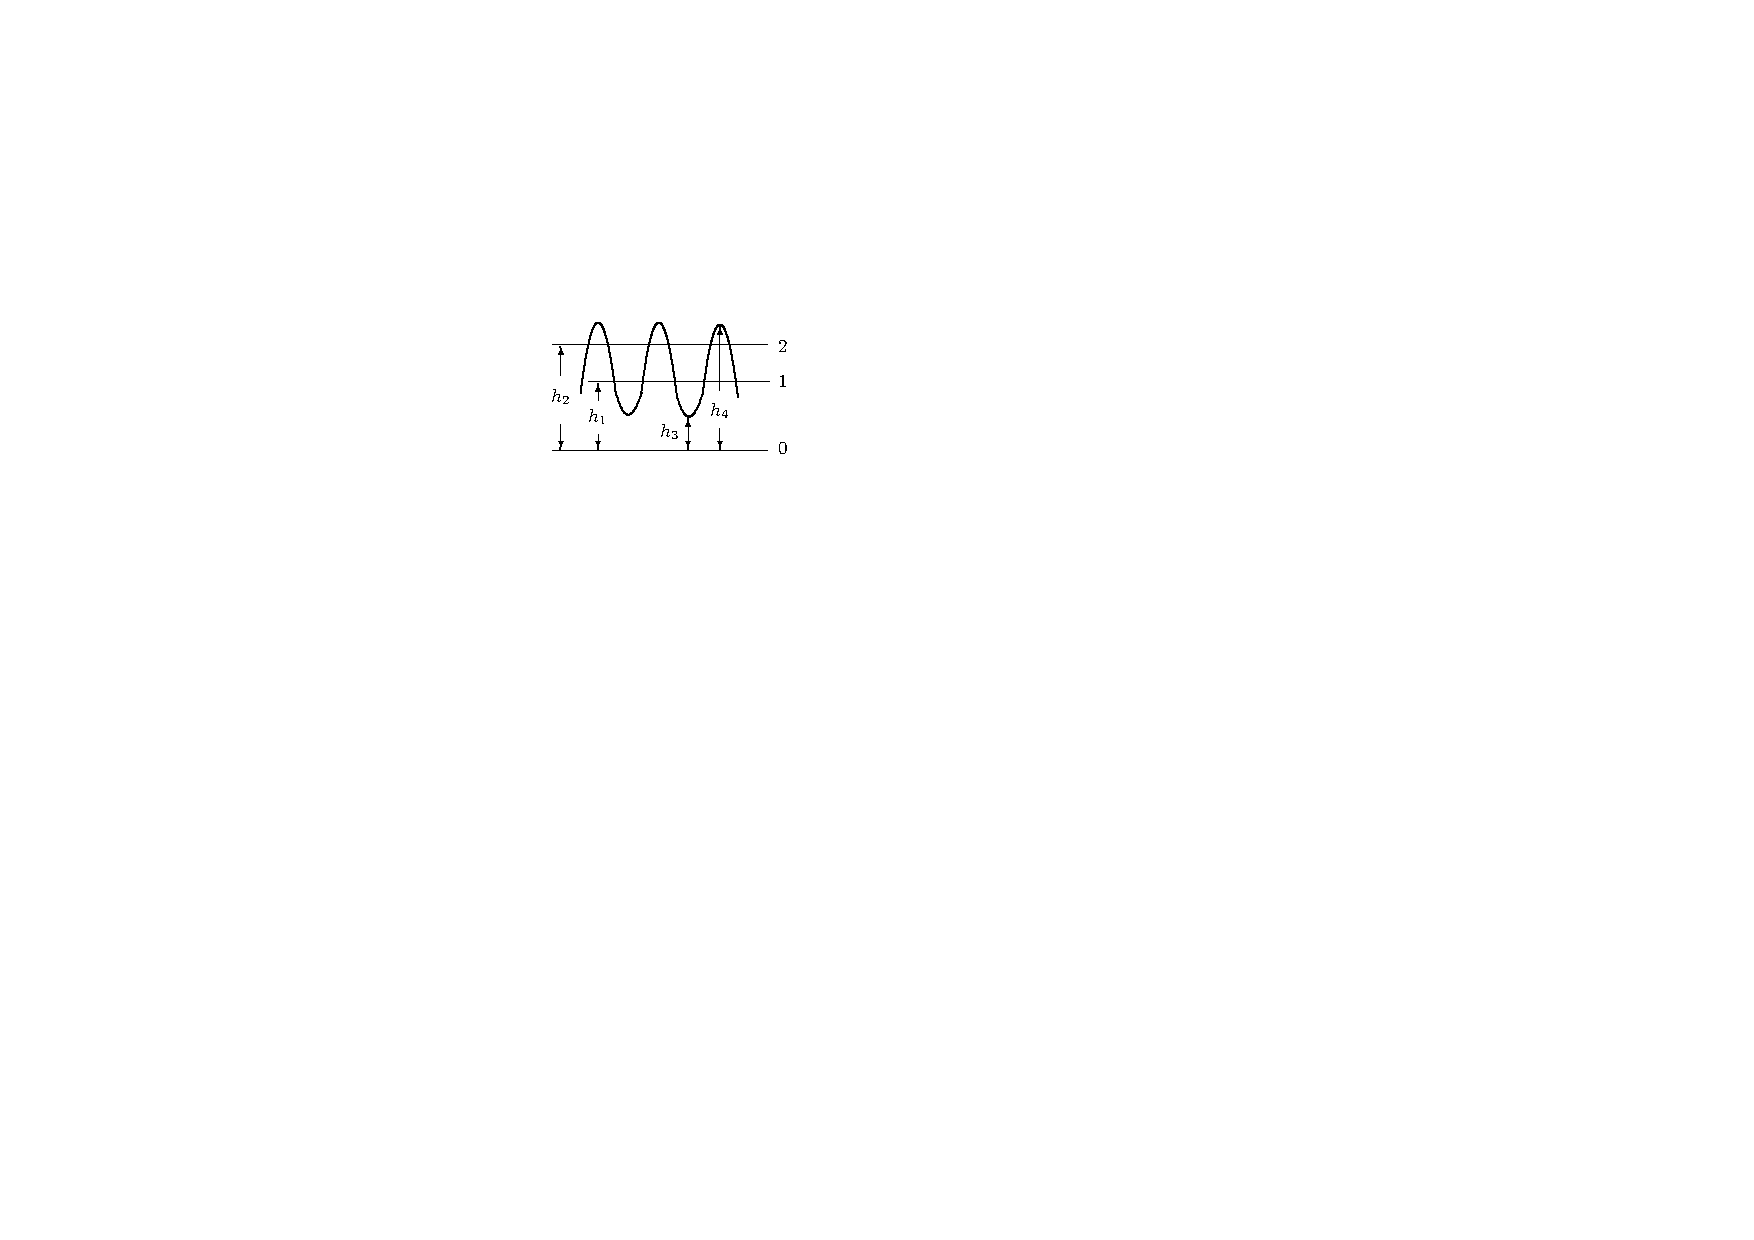
\includegraphics[scale=1.5]{1.pdf}
	\end{figure}
	\begin{equation}
	\delta = \frac{h_1}{h_2}, \; \gamma = \frac{h_4-h_3}{h_4+h_3}.
	\end{equation}	
	
\section{Экспериментальная установка}
	\begin{figure}[H]
		\caption{Схема установки}
		\label{inst}
		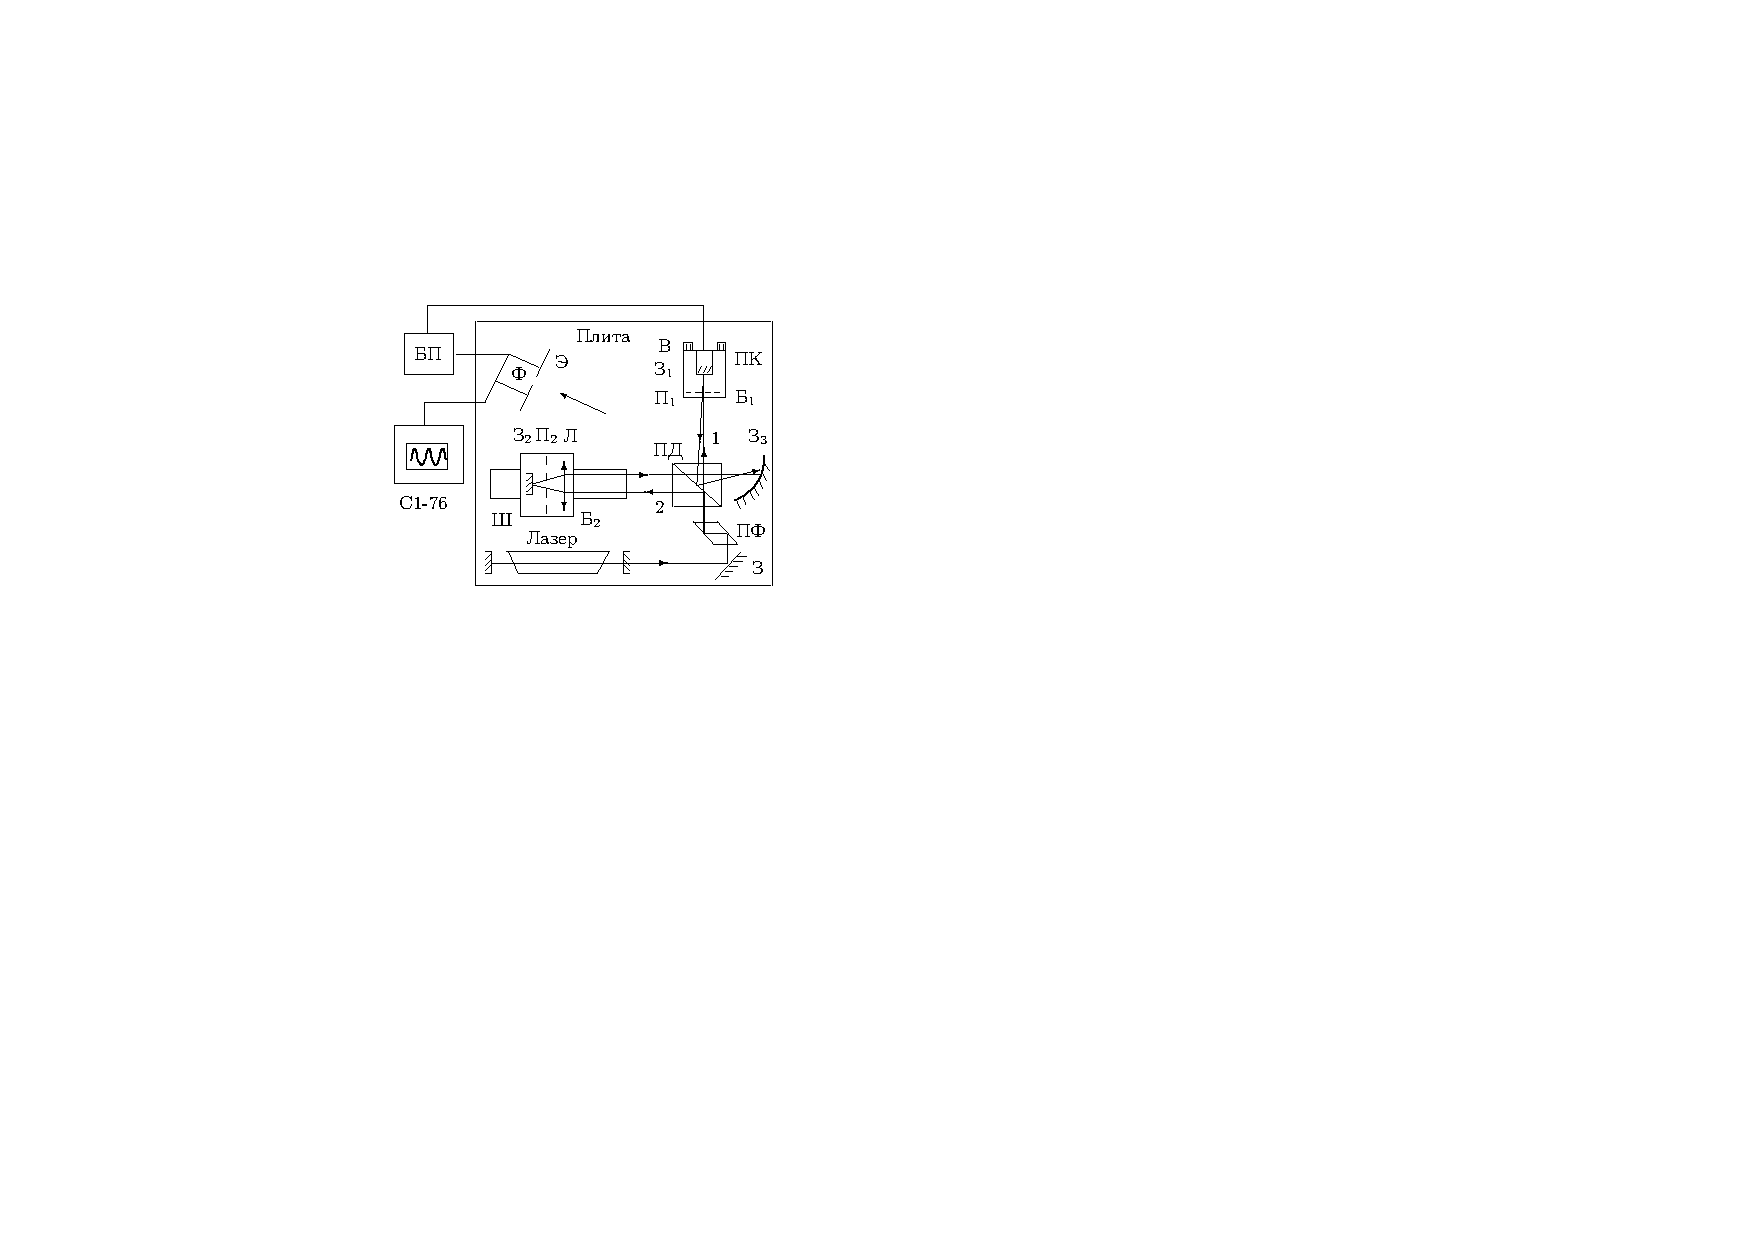
\includegraphics[scale=1.5]{inst.pdf}
	\end{figure}
	Луч 1 проходит поляроид $П_1$, отражается под небольшим углом от зеркала $З_1$, снова проходит
	поляроид $П$ и, частично отражаясь от диагональной плоскости делительной призмы, выходит из интерферометра. Зеркало $З_1$ наклеено на пьезокерамику ПК, которая может осуществлять малые
	колебания зеркала вдоль падающего луча. Поляроид и зеркало с пьезокерамикой собраны в единый блок $Б_1$, который крепится к вертикально стоящей плите. В блоке $Б_1$ имеются юстировочные винты В, которые позволяют регулировать угол наклона зеркала $З_1$ В установке предусмотрена возможность вращения поляроида $П_1$ вокруг луча 1. Угол поворота отсчитывается по шкале, нанесённой на оправу поляроида.
	
	Луч 2 проходит линзу Л, поляроид $П_2$, отражается от зеркала $З_2$, снова проходит поляроид $П_2$, линзу Л и частично выводится делительной призмой из интерферометра. Зеркало $З_2$ установлено в фокальной плоскости линзы Л. Это сделано для того, чтобы падающий и выходящий из системы лучи всегда были параллельны друг другу. Линза Л, поляроид $П_2$ и зеркало $З_2$ собраны в единый блок $Б_2$. Этот блок может перемещаться вдоль луча 2 по штанге Ш, жёстко связанной с плитой интерферометра. Длина штанги 90 см. В установке предусмотрена возможность небольшого перемещения блока $Б_2$ перпендикулярно лучу, что позволяет регулировать расстояние между падающим и выходящим из блока лучами. При измерениях блок $Б_2$ крепится к штанге при помощи двух винтов. Вдоль штанги нанесены деления через один сантиметр. При перемещении блока $Б_2$ вдоль штанги на величину $ l_1 $ геометрическая разность хода между лучами 1 и 2 изменяется на величину $ l = 2l_1 $.
	
	Лучи 1 и 2 накладываются друг на друга и интерферируют вблизи задней грани делительной призмы ПД. Сферическое зеркало $З_3$ с небольшим фокусным расстоянием увеличивает картину интерференционных полос и проецирует её на экран Э.
	
\section{Экспериментальная часть}
	\subsection{Экспериментальные данные}
		\floatsetup[table]{capposition=top}	
		\begin{table}[H]
			\caption{Зависимость видности от угла поворота поляроида при нулевой разности хода.}
			\label{table:exp1}
			\begin{tabular}{|l|l|l|l|l|l|l|l|l|}
				\hline
				$ \alpha $, $ ^\circ $ & $ h_1 $  & $ h_2 $  & $ h_3 $  & $ h_4 $  & $ \gamma $     & $ \delta $    & $ \gamma_1 $   & $ \gamma_3 $   \\ \hline
				0    & 0,8 & 0,8 & 0,8 & 2,5 & 0,515 & 1,00  & 1,00 & 0,515 \\ \hline
				20   & 0,3 & 0,8 & 0,4 & 1,8 & 0,636 & 2,67  & 0,89 & 0,714 \\ \hline
				40   & 0,2 & 2,0   & 1,2 & 3,3 & 0,467 & 10,0 & 0,57 & 0,812 \\ \hline
				60   & 0,2 & 2,0   & 1,4 & 3,0   & 0,364 & 10,0 & 0,57 & 0,632 \\ \hline
				90   & 0,7 & 2,0   & 2,0   & 3,3 & 0,245 & 2,86  & 0,88 & 0,280 \\ \hline
				100  & 1,3 & 2,0   & 2,7 & 3,6 & 0,143 & 1,54  & 0,98 & 0,146 \\ \hline
				110  & 1,6 & 2,0   & 3,3 & 3,7 & 0,057 & 1,25  & 0,99 & 0,057 \\ \hline
				120  & 1,5 & 1,9 & 3,2 & 3,7 & 0,072 & 1,27  & 0,99 & 0,073 \\ \hline
				140  & 0,8 & 0,8 & 1,1 & 2,0   & 0,290 & 1,00  & 1,00 & 0,290 \\ \hline
				-10  & 1,0   & 0,8 & 1,1 & 2,0   & 0,290 & 0,80  & 0,99 & 0,292 \\ \hline
				-20  & 1,1 & 0,7 & 2,2 & 2,5 & 0,064 & 0,64  & 0,97 & 0,065 \\ \hline
			\end{tabular}
		\end{table}
		
		\floatsetup[table]{capposition=top}	
		\begin{table}[H]
			\caption{Зависимость видности от разности хода между лучами}
			\label{table:exp2}
			\begin{tabular}{|l|l|l|l|l|l|l|l|l|}
				\hline
				$x$, см & $h_1$  & $h_2$  & $h_3$  & $h_4$ & $ \gamma $    & $ \delta $   & $ \gamma_1 $   & $ \gamma_2 $    \\ \hline
				8      & 1,8 & 1,0   & 1,4 & 3,0   & 0,364 & 0,56 & 0,96 & 0,737 \\ \hline
				10     & 1,3 & 1,2 & 1,5 & 3,5 & 0,400 & 0,92 & 1,00 & 0,777 \\ \hline
				16     & 0,8 & 0,8 & 0,8 & 2,5 & 0,515 & 1,00 & 1,00 & 1,000 \\ \hline
				18     & 0,7 & 0,7 & 0,7 & 2,0   & 0,481 & 1,00 & 1,00 & 0,935 \\ \hline
				21     & 0,7 & 0,7 & 0,7 & 1,9 & 0,462 & 1,00 & 1,00 & 0,896 \\ \hline
				24     & 0,6 & 0,7 & 0,9 & 1,9 & 0,357 & 1,17 & 1,00 & 0,695 \\ \hline
				28     & 1,3 & 2,0   & 2,8 & 3,8 & 0,152 & 1,54 & 0,98 & 0,301 \\ \hline
				32     & 1,4 & 1,7 & 2,9 & 3,1 & 0,033 & 1,21 & 1,00 & 0,065 \\ \hline
				38     & 0,6 & 1,0   & 1,4 & 1,7 & 0,097 & 1,67 & 0,97 & 0,194 \\ \hline
				46     & 0,6 & 1,1 & 1,6 & 1,9 & 0,086 & 1,83 & 0,96 & 0,174 \\ \hline
				54     & 0,6 & 1,2 & 1,8 & 2,0   & 0,053 & 2,00 & 0,94 & 0,108 \\ \hline
				62     & 0,6 & 1,5 & 2,0   & 2,2 & 0,048 & 2,50 & 0,90 & 0,102 \\ \hline
				68     & 0,4 & 2,3 & 2,5 & 2,9 & 0,074 & 5,75 & 0,71 & 0,202 \\ \hline
				70     & 0,4 & 2,0   & 2,0   & 2,7 & 0,149 & 5,00 & 0,75 & 0,388 \\ \hline
				72     & 0,5 & 1,7 & 1,6 & 2,7 & 0,256 & 3,40 & 0,84 & 0,592 \\ \hline
				74     & 0,5 & 1,1 & 1,0   & 2,1 & 0,355 & 2,20 & 0,93 & 0,743 \\ \hline
				76     & 0,4 & 1,9 & 1,4 & 3,2 & 0,391 & 4,75 & 0,76 & 1,002 \\ \hline
				78     & 0,4 & 1,0   & 0,7 & 2,1 & 0,500 & 2,50 & 0,90 & 1,074 \\ \hline
				80     & 0,3 & 2,0  & 1,4 & 3,1 & 0,378 & 6,67 & 0,67 & 1,089 \\ \hline
				82     & 0,3 & 1,7 & 1,2 & 2,7 & 0,385 & 5,67 & 0,71 & 1,045 \\ \hline
				84     & 0,3 & 0,8 & 0,6 & 1,6 & 0,455 & 2,67 & 0,89 & 0,991 \\ \hline
			\end{tabular}
		\end{table}
	\newpage
	\subsection{Обработка результатов}
		Рассчитаем коэффициент $ \gamma_3$, и построим график  $ \gamma_3(\cos\alpha) $ и $ \gamma_3(\cos^2\alpha) $:
		\begin{figure}[h!]
			\begin{floatrow}
				\ffigbox[\FBwidth]{\caption{Зависимость $\gamma_3$ от $\cos \alpha$.}\label{fig:Graph1}}%
				{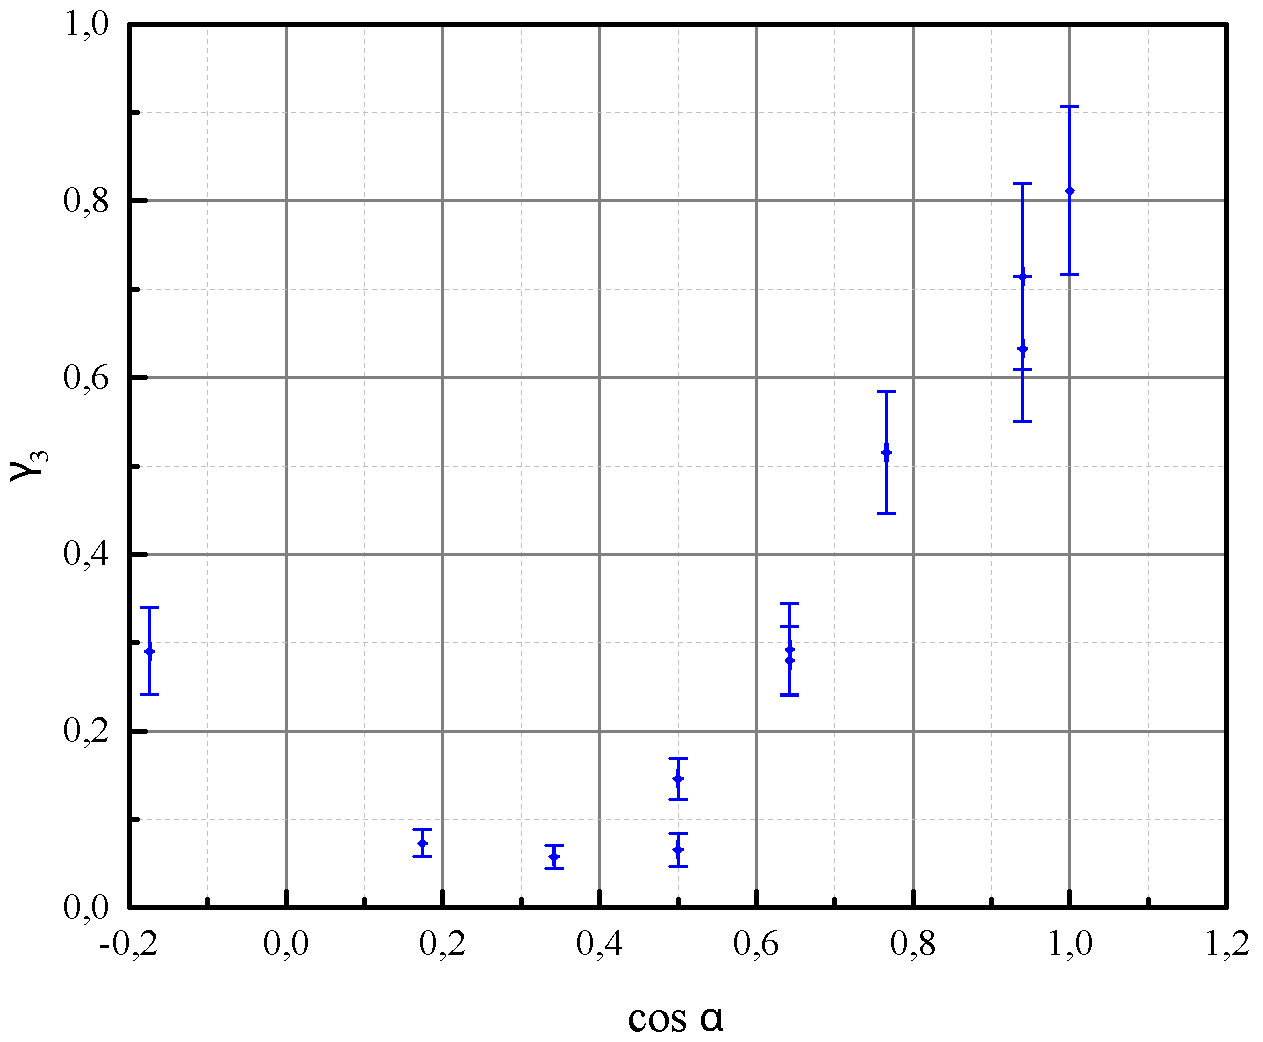
\includegraphics[width=8cm,height=7cm]{graph1}}
				\ffigbox[\FBwidth]{\caption{Зависимость $\gamma_3$ от $\cos^2 \alpha$.}\label{fig:Graph2}}%
				{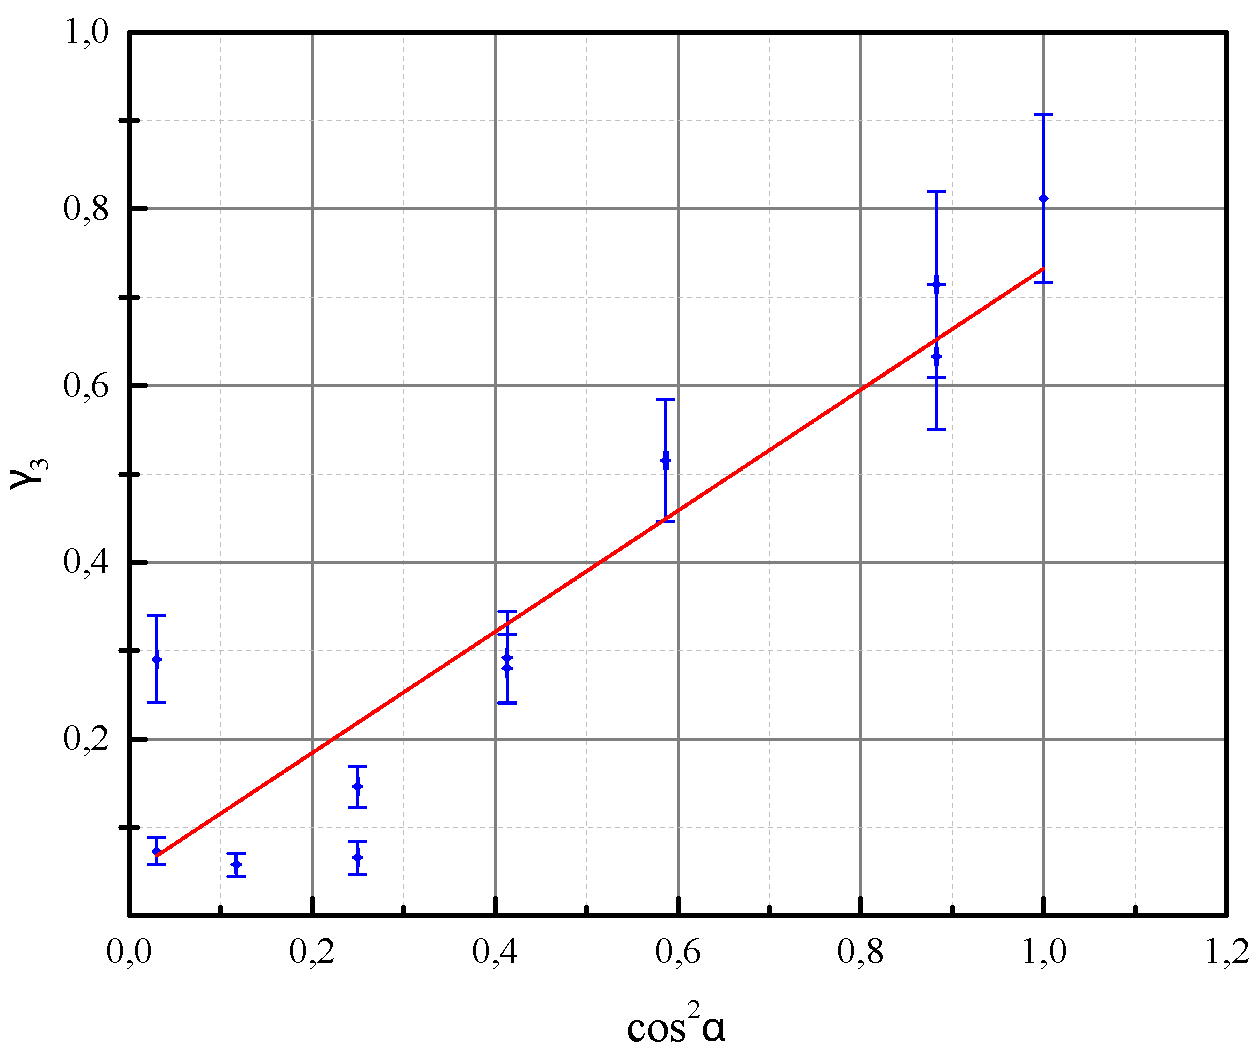
\includegraphics[width=8cm,height=7cm]{graph2}}         
			\end{floatrow}
		\end{figure}
		
		Рассчитаем коэффициент $\gamma_2$ и построим график зависимости видности $\gamma_2(x)$ от координаты блока Б2:
		\begin{figure}[h!]
			\begin{floatrow}
				\ffigbox[\FBwidth]{\caption{Зависимость $\gamma_2 = \gamma_2(x)$.}\label{fig:Graph3}}%
				{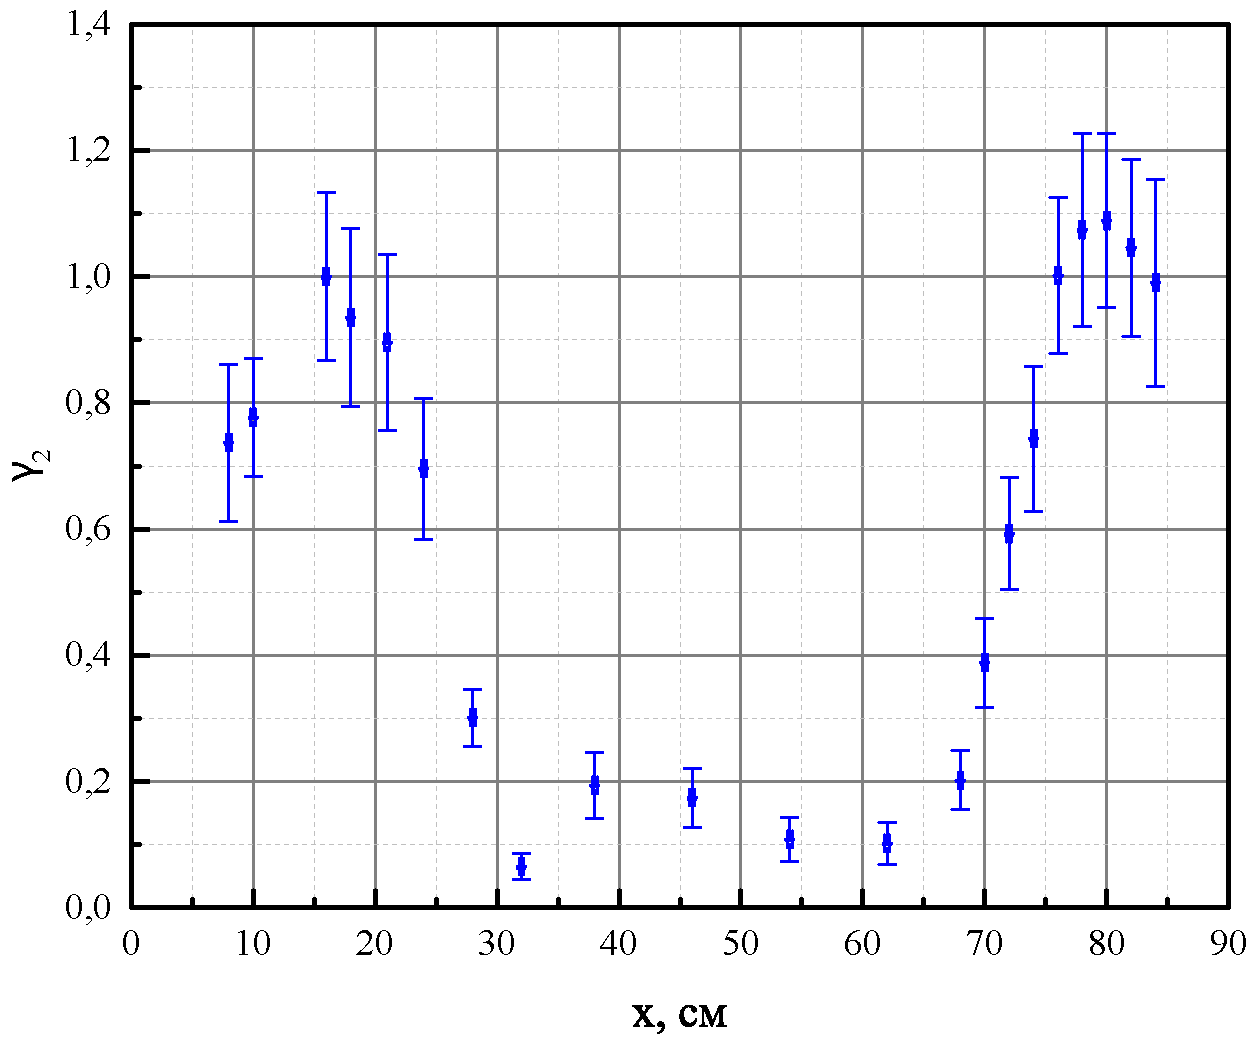
\includegraphics[width=8cm,height=7cm]{graph3}}       
			\end{floatrow}
		\end{figure}
	
		По полученному графику оценим расстояние $L$ между зеркалами оптического резонатора лазера и межмодовое расстояние $\Delta\nu$:
		\begin{equation}
		L = (32,0\pm 0,3) \; \text{см}, \; \Delta\nu = \frac{c}{2L} = (4,69\pm 0,06)\cdot 10^8 \; \text{Гц}.
		\end{equation}
		
		Определим полуширину $l_{1/2}$ отдельного максимума на половине высоты и рассчитаем диапазон частот $2\Delta F$, в котором происходит генерация продольных мод:
		\begin{equation}
		l_{1/2} \approx 8\; \text{см}, \; 2\Delta F = \frac{2c\sqrt{\ln 2}}{\pi l_{1/2}} \approx 1,33\cdot 10^9 \; \text{Гц}.
		\end{equation}
		
	    Оценим число генерируемых лазером продольных мод:
		\begin{equation}
		N = 1 + \frac{2\Delta F }{\Delta\nu} \approx 4.
		\end{equation}

\newpage
\section{Выводы}
	Точки графика рис.~\ref{fig:Graph2} намного лучше ложатся на прямую, чем точки графика рис.~\ref{fig:Graph1}. Это связано с хаотически меняющимся направлением линейной поляризации источника. Действительное значение расстояния между зеркалами составляет 65 см, что в два раза больше полученного нами. По рис. \ref{fig:Graph3} можно предположить, что число мод равно 3.
	
	
	
	
	
	
	
	
	
	
	
	
	
	
	
	
	
	
	
	
	
	
	
	
\end{document}